%% Research Notes of the AAS (RNAAS) Manuscript
%% Note: Per RNAAS guidelines, DO NOT enable the `linenumbers` class option.
%% If compiling on an older Overleaf TeX Live image lacking AASTeX v7, switch to:
%%   \documentclass[RNAAS]{aastex631}
%% and change \bibliographystyle{aasjournalv7} to \bibliographystyle{aasjournal}.
\documentclass[RNAAS]{aastex7}

\usepackage{amsmath}
\usepackage{graphicx}
\usepackage{hyperref}

\begin{document}

\title{Numerical Validation and Reference Lightcone Benchmark for In-Flight Distributed Stellar Population Synthesis with \texttt{specsynth}}

\author[0009-0006-1590-1356]{Sankar Ganesh}
\affiliation{Independent Researcher}
\email{sankarganesh.astro@example.org} % TODO: replace with your preferred contact email before submission

\begin{abstract}
Forward-modeling broadband photometry for $10^6$--$10^9$ simulated galaxies in surveys such as Rubin LSST, Euclid, and Roman creates severe spectral storage and memory bottlenecks. I present empirical validation, multi-platform benchmarks, and a public 100,000-galaxy lightcone reference catalog (\texttt{DOI: 10.57967/hf/11635}) for \texttt{specsynth}, an open-source Dask/Zarr/CuPy engine that evaluates Charlot \& Fall dust, Planck~2018 luminosity-distance scaling, Madau IGM transmission, and 16-band photometric projection in-flight without writing intermediate spectra. Against independent \texttt{float64} baselines, \texttt{float32} streaming achieves a maximum relative spectral error of $9.87\times 10^{-7}$, photometric residuals below $3.0\times 10^{-7}$~mag across JWST, HST, and SDSS bandpasses, constant worker RAM (261.5--261.8~MB across $10^5$--$10^6$ galaxies), and $2.59\times 10^5$~gal~s$^{-1}$ on an NVIDIA Tesla T4 GPU.
\end{abstract}

\keywords{
\uat{Astronomy software}{1855} ---
\uat{Spectral energy distribution}{2129} ---
\uat{Stellar populations}{1622} ---
\uat{Broad band photometry}{184} ---
\uat{Computational methods}{1965}
}

\section{Introduction}

Interpreting wide-field galaxy surveys---including the Vera C. Rubin Observatory Legacy Survey of Space and Time \citep[LSST;][]{ivezic2019lsst}, \textit{Euclid} \citep{mellier2025euclid}, and the Nancy Grace Roman Space Telescope \citep{akeson2019wfirst}---requires forward-modeling synthetic photometry for millions to billions of simulated galaxies. Retaining full intermediate spectra ($W \approx 2{,}000$--$10{,}000$ wavelength bins) before integrating into 5--16 photometric bandpasses generates multi-terabyte temporary arrays and frequently exhausts host RAM or POSIX scratch storage.

To quantify whether mixed-precision, out-of-core matrix streaming can eliminate intermediate spectral storage without compromising photometric precision, I validate \texttt{specsynth} v1.0.0\footnote{\url{https://github.com/SankarGaneshb/specsynth}}, an MIT-licensed Python execution engine built on chunked Zarr storage, Dask task graphs \citep{rocklin2015dask}, OpenBLAS, and optional CuPy GPU contractions \citep{okuta2017cupy}. In this Research Note, I summarize its verified numerical fidelity, empirical throughput across CPU, GPU, and cloud Kubernetes hardware, and the accompanying public 100,000-galaxy lightcone reference dataset \citep{sankar_ganesh_bala_krishnan_2026}.

\section{In-Flight Forward-Modeling Pipeline}

For each streamed chunk of $N_{\text{chunk}}$ galaxies, \texttt{specsynth} caches a pre-compiled Simple Stellar Population (SSP) basis ($K\times W$) on each worker and evaluates composite stellar flux density under the \citet{charlot2000simple} two-component dust model:
\begin{equation}
F_g(\lambda) = D_g(\lambda)\!\left[\sum_{k\in\text{old}}\mathrm{SFH}[g,k]\,\mathrm{SSP}[k,\lambda] + B_g(\lambda)\sum_{k\in\text{young}}\mathrm{SFH}[g,k]\,\mathrm{SSP}[k,\lambda]\right],
\end{equation}
where populations younger than $10^7$~yr receive additional birth-cloud attenuation $B_g(\lambda)$ atop diffuse interstellar medium attenuation $D_g(\lambda)$. Each chunk executes as two dense \texttt{float32} GEMM operations, followed by \texttt{FlatLambdaCDM} luminosity-distance dimming ($F_\lambda = L_{\lambda/(1+z)}/[4\pi D_L^2(1+z)]$) and \citet{madau1995radiative} intergalactic medium (IGM) transmission. Bandpass integration contracts chunk spectra directly against a \texttt{float64}-normalized filter matrix ($\mathbf{Phot} = \mathbf{F}_{\text{chunk}}\mathbf{M}_{\text{filter}}$) in L3 cache or GPU VRAM and immediately discards $\mathbf{F}_{\text{chunk}}$, reducing output storage by $>99.9\%$ while bounding worker memory strictly to $O(N_{\text{chunk}} \times W)$. An integrated four-tier quality sentry (\texttt{specsynth.sentry}) checks finiteness, flux positivity, dust energy conservation, $D_n(4000)$ breaks, UV continuum slopes, and population color collapse during execution.

\section{Empirical Validation and Multi-Platform Benchmarks}

All verification metrics are archived in machine-readable JSON manifests inside the repository and summarized in Figure~\ref{fig:validation}.

\begin{figure}[ht!]
\centering
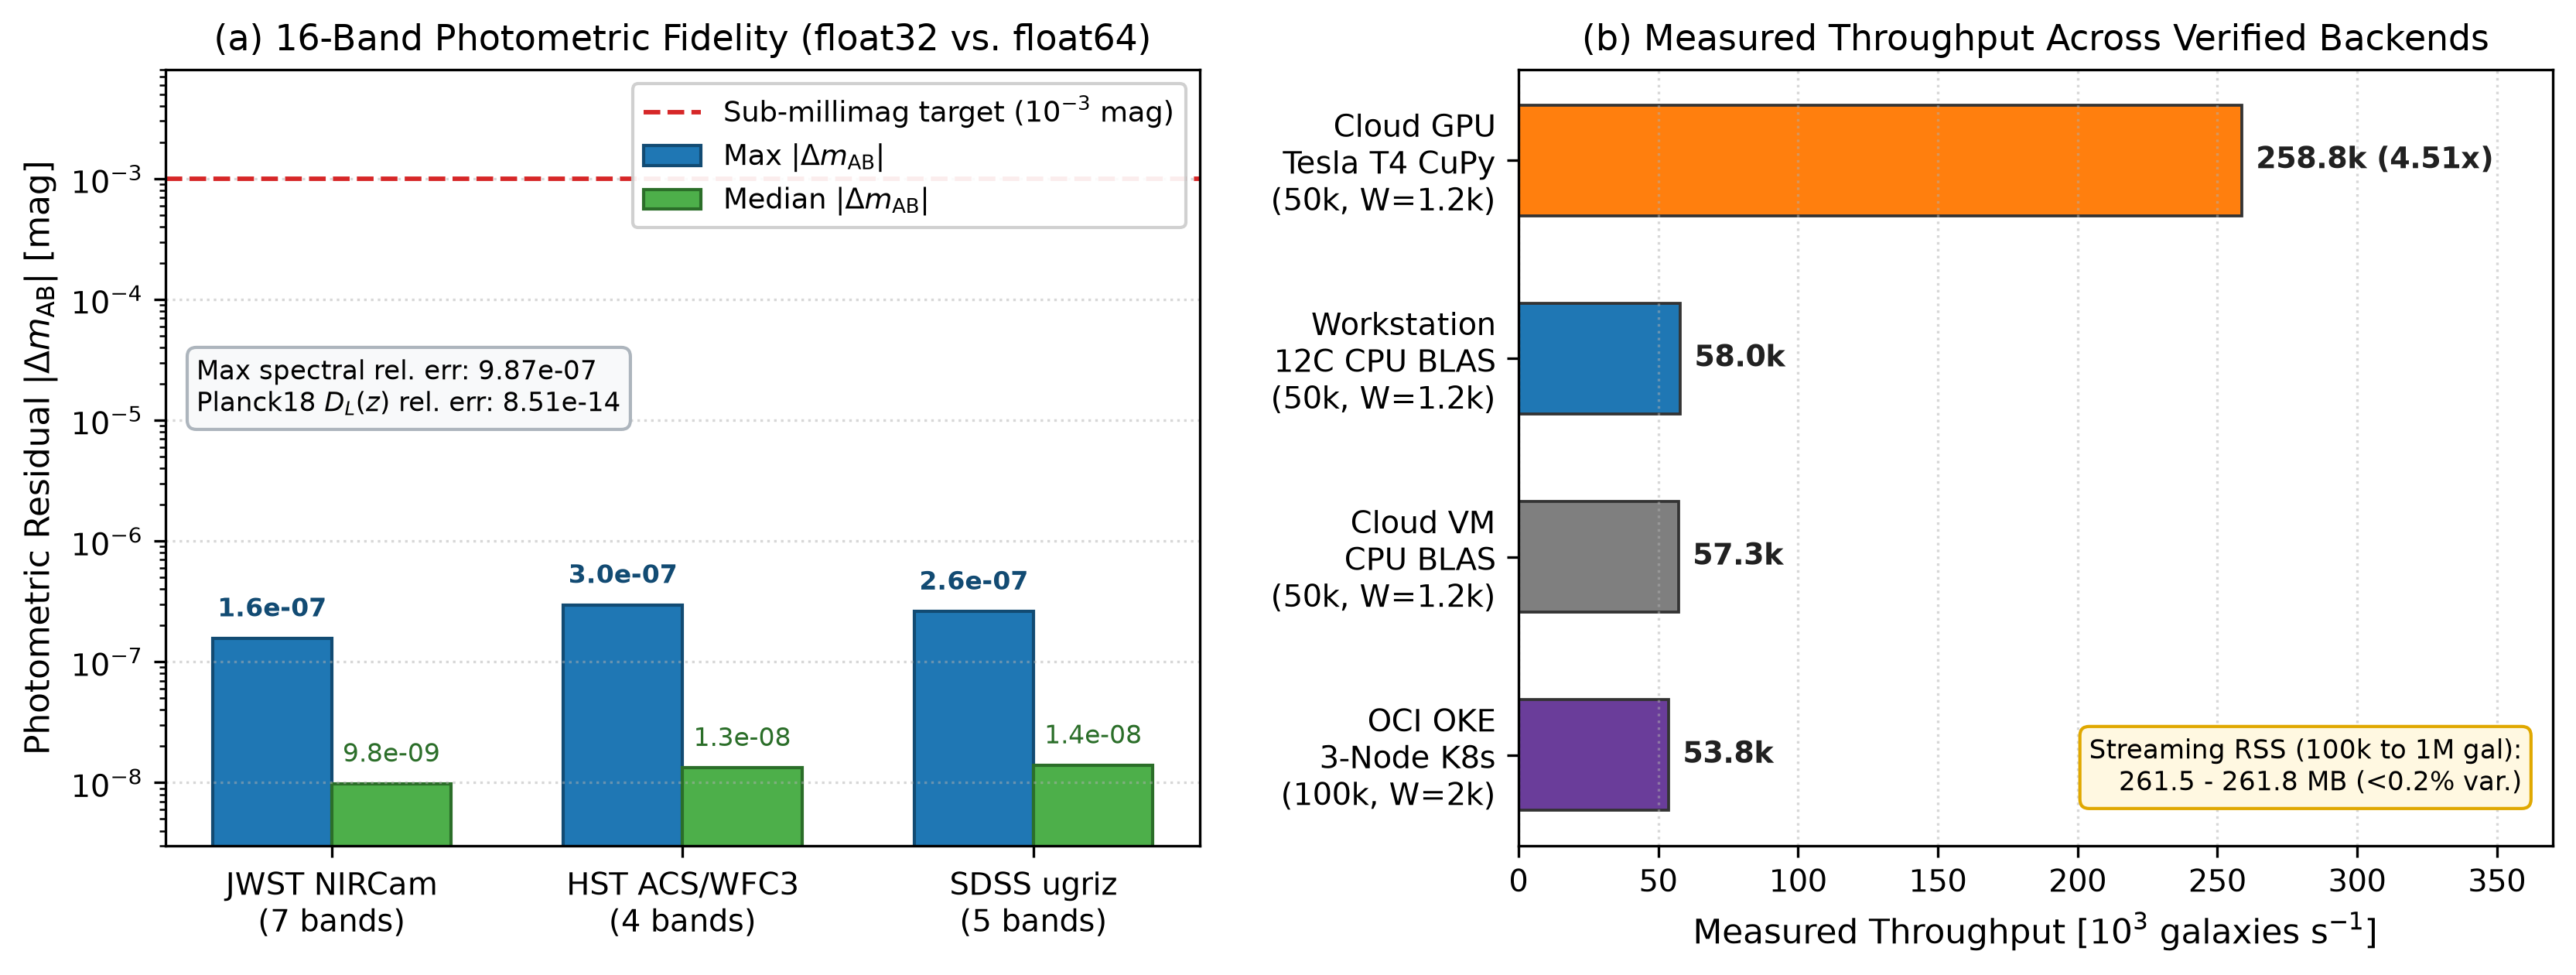
\includegraphics[width=\textwidth]{fig1_validation.png}
\caption{Empirical numerical validation and execution throughput of \texttt{specsynth} v1.0.0. (a)~Maximum and median absolute AB magnitude residuals ($|\Delta m_{\mathrm{AB}}|$) between \texttt{float32} in-flight contraction and an independent serial \texttt{float64} reference across 16 calibrated JWST NIRCam, HST ACS/WFC3, and SDSS bandpasses for a 500-galaxy IllustrisTNG-like sample at $z=2.0$; inset reports the maximum relative spectral error ($9.87\times 10^{-7}$) and Planck~2018 luminosity-distance error ($8.51\times 10^{-14}$). (b)~Measured throughput across verified execution backends: 3-node Oracle Cloud Kubernetes cluster ($53.8\times 10^3$~gal~s$^{-1}$), cloud VM CPU ($57.3\times 10^3$~gal~s$^{-1}$), 12-core workstation CPU ($58.0\times 10^3$~gal~s$^{-1}$), and NVIDIA Tesla T4 GPU ($258.8\times 10^3$~gal~s$^{-1}$, $4.51\times$ speedup); inset confirms constant streaming worker RSS (261.5--261.8~MB) across $10^5$--$10^6$ galaxies.\label{fig:validation}}
\end{figure}

\textit{Spectral, Photometric, and Cosmological Accuracy.}---Against an independent serial \texttt{float64} engine over 2,000 galaxies ($K=60$, $W=1{,}200$), \texttt{float32} streaming yields a maximum relative spectral error of $9.87\times 10^{-7}$, mean relative error of $8.77\times 10^{-8}$, median relative error of $7.21\times 10^{-8}$, and RMSE of $2.24\times 10^{-11}$. Using \texttt{scripts/cross\_validate\_sps.py} on a 500-galaxy IllustrisTNG-like population at $z=2.0$ across all 16 calibrated STScI/SDSS bandpasses, maximum photometric residuals stay well below the $10^{-3}$~mag survey requirement: $1.57\times 10^{-7}$~mag (JWST NIRCam, 7 bands), $2.96\times 10^{-7}$~mag (HST ACS/WFC3, 4 bands), and $2.61\times 10^{-7}$~mag (SDSS $ugriz$, 5 bands), with median residuals of $0.98$--$1.39\times 10^{-8}$~mag. Over $z\in[0.05,6.0]$, luminosity distances agree with independent 2,000-node FLRW quadrature to $8.51\times 10^{-14}$ (Planck~2018) and $8.23\times 10^{-14}$ (concordance $\Lambda$CDM).

\textit{Hardware Throughput and Memory Boundedness.}---Across five timed runs on a standardized workload ($N=50{,}000$, $K=60$, $W=1{,}200$), workstation CPU BLAS achieves $57{,}978$~gal~s$^{-1}$ ($0.862\pm 0.058$~s; 17.1~GFLOPS), cloud Linux CPU BLAS achieves $57{,}344$~gal~s$^{-1}$ ($0.872\pm 0.025$~s), and an NVIDIA Tesla T4 GPU via CuPy (CUDA~12.2) reaches $258{,}812$~gal~s$^{-1}$ ($0.193\pm 0.004$~s; 76.4~GFLOPS, a $4.51\times$ measured speedup). Distributed cloud execution on a 3-node Oracle Container Engine for Kubernetes (OKE) cluster synthesizes 100,000 galaxies ($K=120$, $W=2{,}000$, 7 JWST bands, $z=2.0$, Madau IGM) in 1.86~s ($53{,}814$~gal~s$^{-1}$; max relative error $8.16\times 10^{-7}$). Kernel working-set tracking (\texttt{psutil}) while streaming $10^5$ to $10^6$ galaxies in 20,000-galaxy chunks confirms flat peak worker RSS of 261.5--261.8~MB ($<0.2\%$ variance, zero disk spill) versus 14.9~GB for monolithic $W=4{,}000$ spectra.

\section{Public 100,000-Galaxy Reference Benchmark Catalog}

To support reproducible cross-code photometric testing, I archived \texttt{specsynth-benchmark-100k} on Hugging Face under permanent DOI \href{https://doi.org/10.57967/hf/11635}{\texttt{10.57967/hf/11635}} \citep{sankar_ganesh_bala_krishnan_2026}. The catalog provides 100,000 mock galaxies spanning a cosmological lightcone ($z\in[0.05, 3.8]$) with stellar masses, star formation history parameters, Charlot \& Fall dust optical depths, and \texttt{float64} ground-truth photometry across all 16 calibrated JWST, HST, and SDSS bandpasses in Parquet and Zarr formats. All source code, reproduction scripts, and optional live \texttt{python-fsps}/\texttt{DSPS} cross-validation hooks are publicly available on GitHub; a comprehensive software architecture paper will follow as the package matures.

\begin{acknowledgments}
I thank the developers of Dask, Zarr, NumPy, CuPy, and Astropy, and the teams behind public SSP libraries. Generative AI tools assisted with code scaffolding and manuscript editing; I verified all equations, numerical benchmarks, and text.
\end{acknowledgments}

\bibliography{references}{}
\bibliographystyle{aasjournalv7}

\end{document}
